%        File: DesignDocument.tex
%     Created: 一 3月 26 01:00 下午 2018 C
% Last Change: 一 3月 26 01:00 下午 2018 C
%
\documentclass[UTF8,noindent]{ctexart}
\usepackage[a4paper,left=2.0cm,right=2.0cm,top=2.0cm,bottom=2.0cm]{geometry}
\usepackage{hyperref}
\usepackage{url}
\usepackage{graphicx}
\usepackage{amsmath}
\usepackage{amssymb}
\usepackage{enumitem}
\usepackage{tikz}
\usepackage{float}
\usepackage{xeCJK}
\usepackage{listings}
\usepackage{xcolor}
\lstset{language = c,numbers=left, showstringspaces=false,keywordstyle= \color{ blue!70 },commentstyle=\color{red!50!green!50!blue!50}, frame=shadowbox, rulesepcolor= \color{ red!20!green!20!blue!20 } 
} 
\CTEXsetup[format={\Large\bfseries}]{section}
\usetikzlibrary{graphs}
%\newtheorem*{lemma}{Lemma}
\title{\CJKfamily{zhkai}计算机网络研讨课实验报告}
\author{{\CJKfamily{zhkai}冯吕}\ $2015K8009929049$}
\date{\today}
\begin{document}
\maketitle
\zihao{5}
\CJKfamily{zhsong}
%\begin{center}
%  \begin{tabular}{|p{15cm}|}
%    \hline
\section{{\CJKfamily{zhhei}实验题目}}网络传输机制实验二
%\hline
\section{{\CJKfamily{zhhei}实验内容}}
\begin{itemize}
  \item 在本次实验中,需要实现$TCP$数据收发功能, 使得节点之间能够在无丢包网络环境中传输数据。
	\item 运行给定拓扑网络,在$h_1$和 $h_2$上分别运行$tcp\_stack$,验证数据收发功能是否正确。
\end{itemize}
\section{{\CJKfamily{zhhei}实验流程}}
本次实验中,需要实现数据收发功能,实现底层的$tcp\_sock\_write$和$tcp\_sock\_read$
\subsection{$tcp\_sock\_write$}
$tcp\_sock\_write$函数将上层应用$buffer$中存储的数据封装成数据包发送出去,然后需要等待$wait\_send$:

\begin{lstlisting}
int tcp_sock_write(struct tcp_sock *tsk, char *buf, int len){

	int data_len = min(len, 1500 - ETHER_HDR_SIZE
	- IP_BASE_HDR_SIZE - TCP_BASE_HDR_SIZE);
	int pkt_size = ETHER_HDR_SIZE + IP_BASE_HDR_SIZE
	+ TCP_BASE_HDR_SIZE + data_len;

	char *packet = (char *) malloc (pkt_size);
	memset(packet, 0, pkt_size);
	memcpy(packet + ETHER_HDR_SIZE+IP_BASE_HDR_SIZE+
	TCP_BASE_HDR_SIZE, buf, data_len);

	tcp_send_packet(tsk, packet, pkt_size);

	sleep_on(tsk->wait_send);

	return data_len;
}
\end{lstlisting}

对端收到发送过去的数据包后,将数据包中的数据写入$rcv\_buf$中,然后回复$ACK$,同时$wake\_up$ $\ wait\_recv$。由于数据读写可能会发生冲突,因此,需要通过锁对$rcv\_buf$进行互斥访问。

当收到对端发送回来的$ACK$后,再$wake\_up$ $\ wait\_send$。

\subsection{$tcp\_sock\_read$}
$tcp\_sock\_read$函数则是从$rcv\_buf$中读取数据到上层应用$buffer$中,如果$rcv\_buf$为空,则$wait\_rcv$,等到收到数据后$wake\_up$:
\begin{lstlisting}
int tcp_sock_read(struct tcp_sock *tsk, char *buf, int len){
	pthread_mutex_lock(&tsk->rcv_buf->rw_lock);
	int not_sleep = 1;

	if (ring_buffer_empty(tsk->rcv_buf)){
		pthread_mutex_unlock(&tsk->rcv_buf->rw_lock);
		not_sleep = 0;
		sleep_on(tsk->wait_recv);
	}
	if (!not_sleep){
		pthread_mutex_lock(&tsk->rcv_buf->rw_lock);
	}
	int read_len = read_ring_buffer(tsk->rcv_buf, buf, len);
	pthread_mutex_unlock(&tsk->rcv_buf->rw_lock);
	return read_len;
}
\end{lstlisting}

\subsection{运行实验}
\begin{itemize}
  \item 运行给定网络拓扑;
	\item 在节点$h_1$上运行$tcp$程序,并运行协议栈的服务器模式;
	  \item 在节点$h_2$上运行$tcp$程序,并运行协议栈的客户端模式;
		\item $client$向$server$发送数据,$server$将数据$echo$给$client$;
\end{itemize}

\section{{\CJKfamily{zhhei}实验结果}}
运行$tcp$程序之后,能够成功建立连接,然后收发数据,最后关闭连接:
\begin{figure}[H]
  \centering
  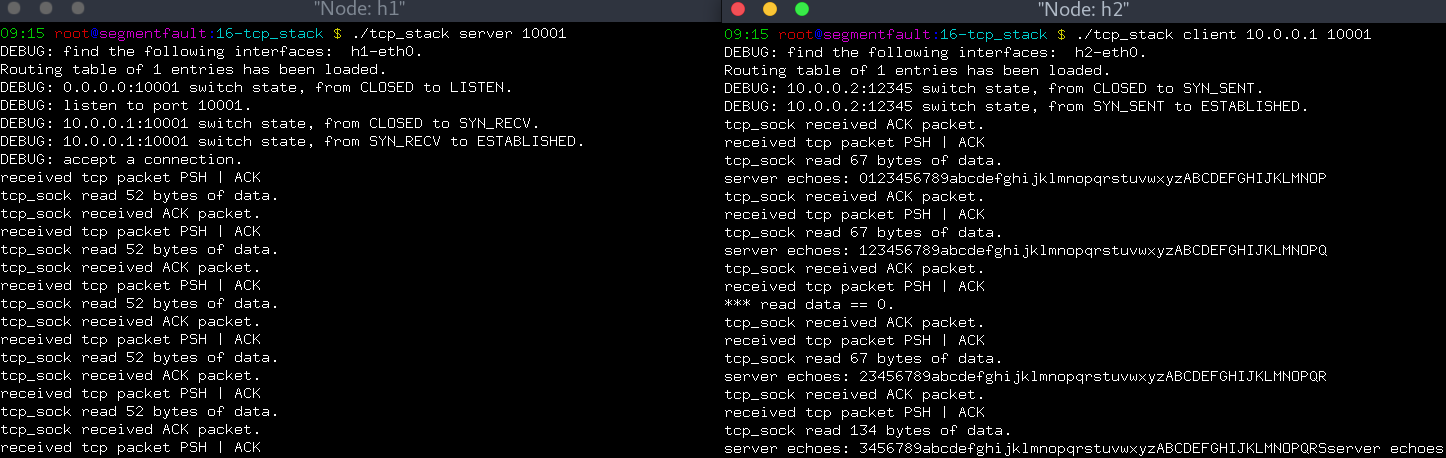
\includegraphics[scale=0.35]{1.png}
  \caption{建立连接$\rightarrow$收发数据}
\end{figure}

\begin{figure}[H]
  \centering
  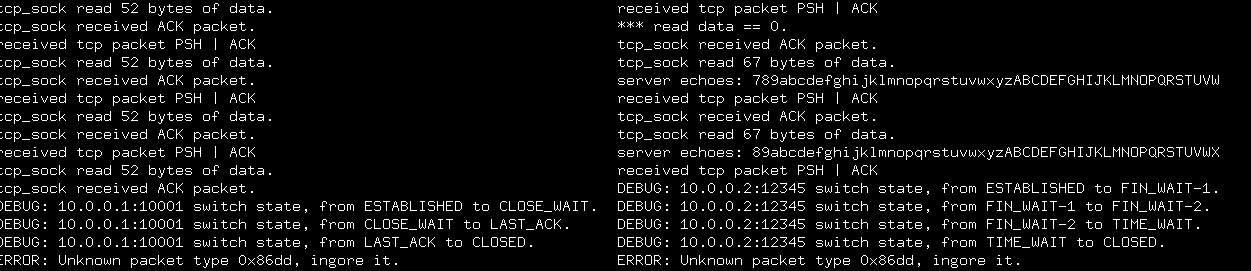
\includegraphics[scale=0.4]{2.png}
  \caption{收发数据$\rightarrow$关闭连接}
\end{figure}


\section{{\CJKfamily{zhhei}结果分析}}

节点建立连接之后能够在不丢包的情况下收发数据。
\end{document}


